\begin{tikzpicture}
    \begin{axis}[
    ybar,
    width=\linewidth, height=5cm,
    ylabel={Accuracy of Map}, ylabel near ticks, ymin=0.5, ymax=1.25,
    ytick={0.6, 0.8, 1},
    xtick={1, 2, 3}, xticklabels={False Positives, False Negatives, Gaussian Noise},
    xmin=0.5, xmax=3.5, xtick pos=left,
    nodes near coords, every node near coord/.append style={rotate=90, anchor=west},
    legend style={at={(0.5,-0.25)}, anchor=north,legend columns=-1},
    bar width=7,
    every node near coord/.append style={
    	/pgf/number format/fixed zerofill,
    	/pgf/number format/precision=4
	}
    ]
        \addplot coordinates {(1, 1.0) (2, 0.9955) (3, 0.8825)};
        \addplot coordinates {(1, 0.9975) (2, 0.97025) (3, 0.5245)};
        \addplot coordinates {(1, 0.983083333333333) (2, 0.99625) (3, 0.697916666666667)};
        \addplot coordinates {(1, 0.9905) (2, 0.9965) (3, 0.701666666666667)};
        \addplot coordinates {(1, 1.0) (2, 0.973) (3, 0.82025)};
        \addplot coordinates {(1, 0.99875) (2, 0.972) (3, 0.579416666666667)};
        \legend{ANG, INT, SPH, PLN, PYR, COM}
    \end{axis}
\end{tikzpicture}

%\begin{tikzpicture}
%	\begin{axis}[width=\linewidth, height=5cm,
%				symbolic x coords={ANG,INT,SPH,PLN,PYR,COM},
%				xtick=data,bar width=20, ybar, colorbar,
%				]
%\addplot+[point meta=explicit, scatter] table[x=IDE,y=ACC,meta=SPE,col sep=semicolon]{
%	IDE;ACC;SPE
%	ANG;0.95954045954046;22.3882783882784
%	INT;0.827922077922078;2.48135198135198
%	SPH;0.887667887667888;18.7967032967033
%	PLN;0.901986901986902;17.5726773226773
%	PYR;0.931401931401931;1.08050283050283
%	COM;0.855033855033855;8.25524475524475
%};
%	\end{axis}
%\end{tikzpicture}

%\begin{tikzpicture}
%    \begin{axis}[
%    width=\linewidth, height=5cm, xmax=2000, 
%    ylabel={Accuracy of Mapping},
%    xlabel={Running Time ($ms$)},
%    scatter/classes={%
%    	ANG-C={mark=square, blue},
%    	DOT-C={mark=square, red},
%    	SPH-C={mark=square, green},
%    	PLN-C={mark=square, black},
%    	PYR-C={mark=square, brown},
%    	COM-C={mark=square, orange},
%    	ANG-F3={mark=triangle, blue},
%    	DOT-F3={mark=triangle, red},
%    	SPH-F3={mark=triangle, green},
%    	PLN-F3={mark=triangle, black},
%    	PYR-F3={mark=triangle, brown},
%    	COM-F3={mark=triangle, orange},
%    	ANG-R2={mark=o, blue},
%    	DOT-R2={mark=o, red},
%    	SPH-R2={mark=o, green},
%    	PLN-R2={mark=o, black},
%    	PYR-R2={mark=o, brown},
%    	COM-R2={mark=o, orange},
%    	ANG-S1={mark=star, blue},
%    	DOT-S1={mark=star, red},
%    	SPH-S1={mark=star, green},
%    	PLN-S1={mark=star, black},
%    	PYR-S1={mark=star, brown},
%    	COM-S1={mark=star, orange}}, xmode=log]
%	
%%    ylabel={$t \ (\si{ms})$}, ylabel near ticks, ymin=10, ymax=100000,
%%    xtick={1, 2, 3}, xticklabels={$\ang{0}$, $\ang{0.0001}$, $\ang{0.01}$},
%%    xlabel={$\sigma$ (degrees)}, xmin=0.5, xmax=3.5, xtick pos=left, point meta=rawy,
%%    nodes near coords, every node near coord/.append style={rotate=90, anchor=west,
%%    /pgf/number format/.cd,fixed,precision=6},
%%    legend style={at={(0.5,-0.35)}, anchor=north,legend columns=-1}
%%    bar width=7, ymode=log, log origin=infty, max space between ticks=20
%%    ]
%		\addplot[scatter, only marks, scatter src=explicit symbolic, forget plot, mark size=3pt] table[meta=label] {
%		x y label
%		9.92823842823843 1.0 ANG-C
%		33.2207792207792 1.0 ANG-F3
%		21.2604895104895 1.0 COM-C
%		0.353313353313353 1.0 DOT-C
%		0.254545454545455 0.996969696969697 DOT-R2
%		15.2309357309357 1.0 PLN-C
%		0.71028971028971 1.0 PYR-C
%		15.3448218448218 1.0 SPH-C
%		8.59815184815185 0.997502497502498 ANG-R2
%		13.4395604395604 0.995504495504495 PLN-R2
%		13.500999000999 0.996503496503496 SPH-R2
%		24.8221778221778 0.992257742257742 PLN-F3
%		27.1603396603397 0.979187479187479 SPH-F3
%		0.506743256743257 0.972777222777223 PYR-R2
%		25.3459040959041 0.881118881118881 ANG-S1
%		14.3966033966034 0.918831168831169 COM-R2
%		6.41033966033966 0.922577422577423 PYR-F3
%		1.14635364635365 0.791708291708292 DOT-F3
%		94.6336163836164 0.826423576423576 COM-F3
%		14.4562937062937 0.718198468198468 PLN-S1
%		15.7287712287712 0.687312687312687 SPH-S1
%		6.30594405594406 0.49050949050949 PYR-S1
%		1.69180819180819 0.138611388611389 DOT-S1
%		64.2407592407592 0.0187312687312687 COM-S1
%		};
%		\addlegendimage{blue,mark=o} \addlegendentry{ANG}
%		\addlegendimage{red,mark=o} \addlegendentry{INT}
%		\addlegendimage{green,mark=o} \addlegendentry{SPH}
%		\addlegendimage{black,mark=o} \addlegendentry{PLN}
%		\addlegendimage{brown,mark=o} \addlegendentry{PYR}
%		\addlegendimage{orange,mark=o} \addlegendentry{COM}
%    \end{axis}
%\end{tikzpicture}